\setlength{\tabcolsep}{5pt}

\begin{table}[!ht]
\small
    \centering
    {\small
    \resizebox{0.7\linewidth}{!}{
        \begin{tabular}{lc cccc}
            \toprule
            {\large$\gamma$} &  %\bfseries{Sampling method}  &
              & $T$ & \bfseries{FID}  $\downarrow$ & \bfseries{IS} $\uparrow$ & \bfseries{NLL} \\
            \midrule
            Exponential & 
            & 4  & 20.84 & 69.7 & 5.86 \\
            Cubic & 
            & 9 & 7.26 & 165.2 & 4.63  \\ 
            Square & 
            & 10 & 6.35 & 179.9 & 4.38  \\ 
            \textbf{Cosine} & 
            & 10 & \textbf{6.06} & \textbf{181.5} & 4.22 \\    
            Linear & 
            & 16 & 7.51 & 113.2 & 3.75  \\
            Square Root &
            & 32 & 12.33 & 99.0 & 3.34 \\  
            Logarithmic  &
            & 72 & 26.12 & 46.7 &  3.08\\
    \bottomrule
    \end{tabular}
    }
    }
    \vspace{-.1cm}
    \caption{\textbf{掩码调度函数的消融结果。}我们报告每个候选调度函数的最佳FID、IS和负对数似然损失。}
    \label{tab:ablation}
\vspace{-.5cm}
\end{table}


% \begin{figure}[!t]
%     \centering
% 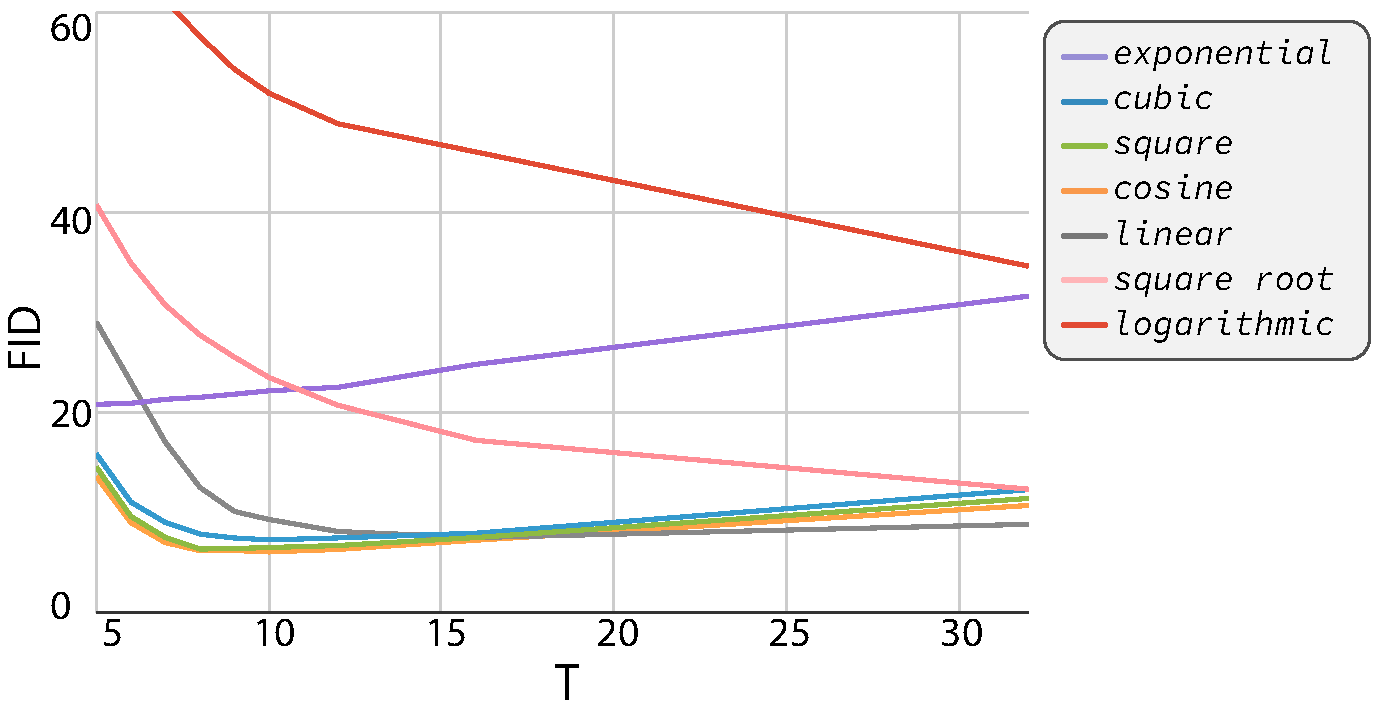
\includegraphics[width=0.8\linewidth]{figures/iteration_vs_fid_scheduling_method.pdf}
%     % \vspace{-25mm}
%     \caption{\textbf{\# of iterations \textit{T}}. Each line graphs a model's FID score against the number of refinement iterations. The lines are named as ''\textit{training distribution - refinement schedule}", e.g. "Linear - Cosine" represents the model that is trained with a linear (i.e. uniform) distribution of mask ratios and uses a cosine refinement schedule.}
%     \label{fig:fidschedule}
% \end{figure}

\begin{figure}[!t]
    \centering
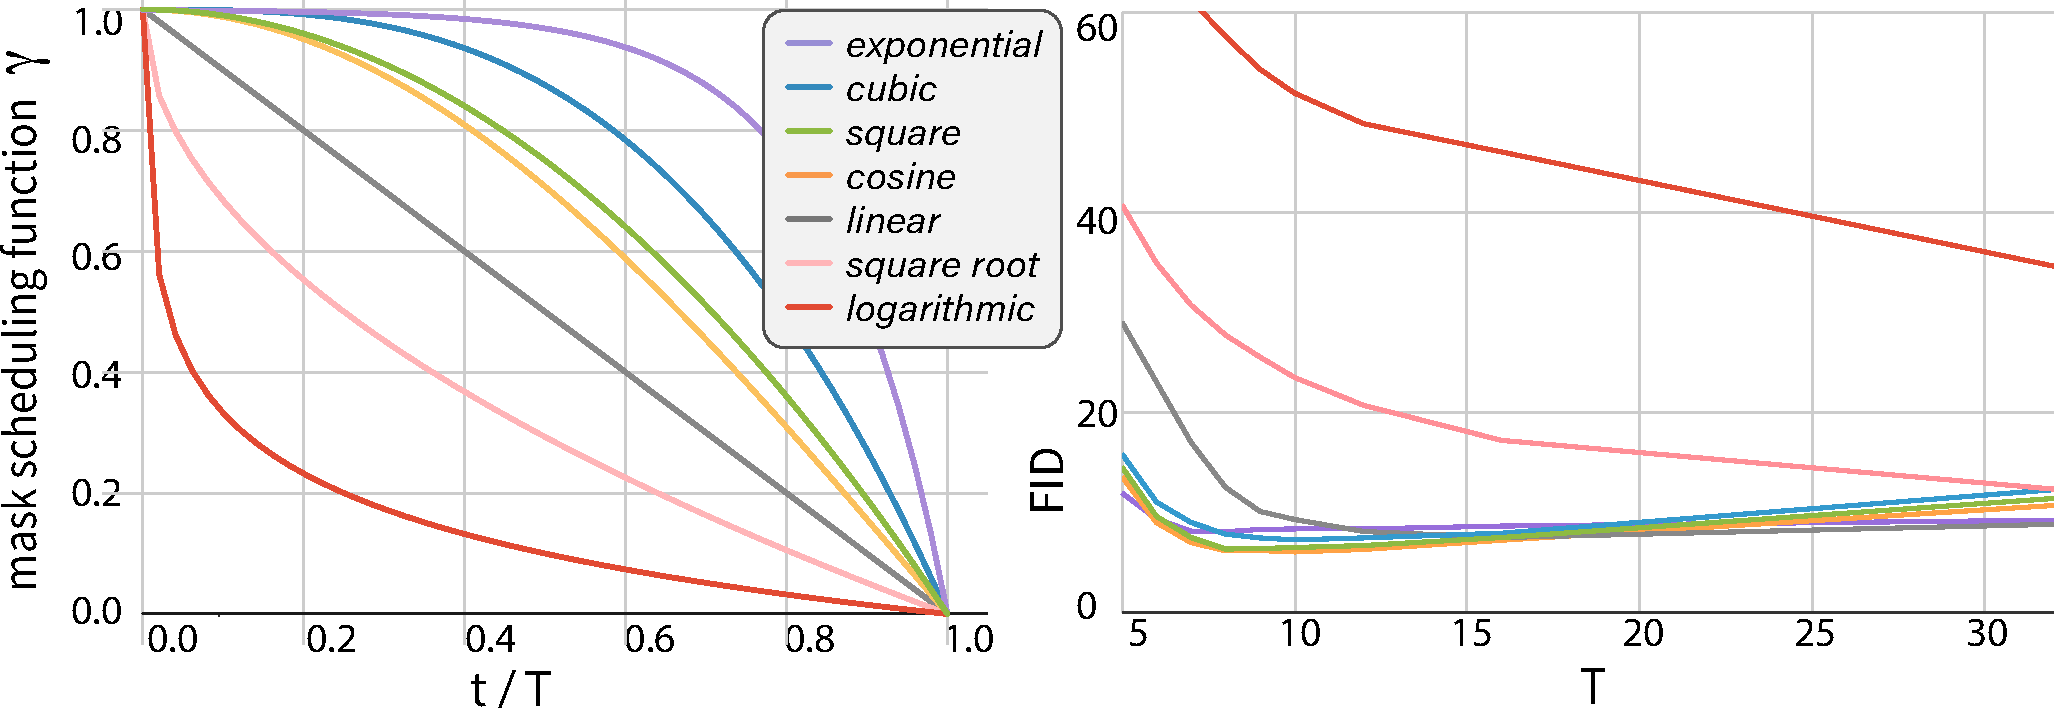
\includegraphics[width=1.\linewidth]{figures/scheduling_func.pdf}
    \vspace{-6mm}
    \caption{\textbf{掩码调度函数的选择} $\gamma (\frac{t}{T})$，以及\textbf{迭代次数\textit{T}}。在左侧，我们可视化了为$\gamma$考虑的七个函数。在右侧，我们展示了模型FID分数与解码迭代次数$T$的线图。在候选者中，我们发现余弦实现了最佳的FID。}
    \label{fig:scheduling}
    \vspace{-5mm}
\end{figure}